% Machine Learning Assignment 3 report, CVPR author kit (https://github.com/cvpr-org/author-kit)
\documentclass[10pt,twocolumn,letterpaper]{article}
\usepackage[pagenumbers]{cvpr}

\usepackage{graphicx}
\usepackage{amsmath,amssymb}
\usepackage{booktabs}
\usepackage{xcolor}
\usepackage{caption}
\graphicspath{{figs/}{../results/}}
\definecolor{cvprblue}{rgb}{0.21,0.49,0.74}
\usepackage[breaklinks,colorlinks,allcolors=cvprblue]{hyperref}
\usepackage{url}

% ====================================================================
% EDIT THESE TWO LINES AFTER THE FINAL COMMIT, THEN RECOMPILE.
\newcommand{\repourl}{PASTE-GITHUB-REPOSITORY-URL-HERE}
\newcommand{\commithash}{PASTE-FINAL-COMMIT-HASH-HERE}
% ====================================================================

\def\confName{CVPR}
\def\confYear{2027}

\title{MLPs, CNNs, Autoencoders, SVMs and Clustering on CIFAR-10\\[2pt]
\large Machine Learning: Assignment 3}

\author{Harsh Prabha Bhaina\\
Roll No.\ M26ECM503, IIT Jodhpur\\
{\small Repository: \url{\repourl}}\\
{\small Final commit: \texttt{\commithash}}}

\begin{document}
\maketitle

% ---------------------------------------------------------------- abstract
\begin{abstract}
We study what different models extract from CIFAR-10 pixels, using one roll-number-seeded split and matched training budgets.
A parameter-matched CNN beats an MLP by 22.2 points (71.57\% vs 49.35\% test).
A fixed pixel permutation removes the whole gap, while a fixed $8{\times}8$ block permutation keeps 59\% of it.
Most of the CNN's advantage therefore comes from structure inside small neighbourhoods.
Adding depth to the MLP at a fixed parameter budget helps by only 2.4--2.6 points.
With 20\% wrong labels, the MLP first predicts the \emph{true} class of mislabelled images and memorises the wrong labels only after its validation peak.
Wider autoencoder bottlenecks reconstruct better and carry more linearly decodable class information.
A denoising autoencoder, however, has lower pixel error yet gives the fixed CNN \emph{lower} accuracy than a plain autoencoder.
On frozen CNN features a linear SVM reaches 71.73\% test accuracy, and $k$-means reaches ARI 0.346.
Clustering and classification rank class pairs similarly (Spearman 0.82) but disagree sharply on bird/deer and automobile/truck.
\end{abstract}

% ---------------------------------------------------------------- setup
\section{Common setup}
\label{sec:setup}
\textbf{Data and split.} CIFAR-10~\cite{krizhevsky2009cifar} has 50,000 training and 10,000 test images ($32{\times}32{\times}3$).
The seed is the digits of the roll number M26ECM503, \texttt{26503}.
\texttt{numpy.random.default\_rng(26503)} drives a stratified split into 45,000 training and 5,000 validation images (exactly 4,500 and 500 per class, checked by assertions).
The split indices, both spatial permutations, the memorisation subset and its relabelling, and the SVM subset are saved in \texttt{results/split.npz}.
Pixels are scaled to $[0,1]$ with no augmentation.
\textbf{Selection.} Every architecture, checkpoint, kernel, $C$ and $k$ is chosen on the validation set (classifiers by validation accuracy, autoencoders by validation MSE, clustering by validation silhouette).
The official test set is loaded only after all choices are fixed (a code comment marks the point).
\textbf{Training.} All networks use PyTorch~\cite{paszke2019pytorch}, Adam, batch 128 and seed 26503.
A 20-epoch classifier run is 7,040 parameter updates.
SVMs and $k$-means use scikit-learn~\cite{pedregosa2011sklearn}.
All results come from one run on an NVIDIA T1000; \cref{tab:reuse} lists which models are reused across questions.

\begin{table}[t]
\centering\footnotesize
\setlength{\tabcolsep}{3pt}
\begin{tabular}{@{}p{0.36\linewidth}lp{0.42\linewidth}@{}}
\toprule
Component & Introduced & Reused in\\
\midrule
Seeded 45k/5k split & Setup & every question\\
Shallow MLP, lr $10^{-3}$ & Q1(a) & Q2 MLP baseline (clean)\\
CNN, clean inputs & Q2(a) & Q3(b) fixed classifier; Q4 features\\
AE, bottleneck 256 & Q3(a) & Q3(b) clean baseline; Q3(c) probe\\
AEs, bottleneck 16/64 & Q3(a) & Q3(c) probes\\
CNN penultimate features & Q4(a) & Q4(b), Q4(c)\\
\bottomrule
\end{tabular}
\caption{Reuse map. Every reused model is the exact validation-selected checkpoint from the question where it was introduced, with no retraining.}
\label{tab:reuse}
\end{table}

% ---------------------------------------------------------------- Q1
\section{Q1: Why MLPs struggle, and when they memorise}
\subsection{Depth versus optimisation}
\textbf{Reason tested.} A one-hidden-layer MLP can only build one level of features, so it may lack the \emph{composition} that images reward.
\textbf{Competing explanation.} A poor step size may stop the MLP from reaching a good solution within the budget. This is an optimisation failure, not a representational one.
\textbf{Design.} We cross depth with learning rate.
A shallow MLP ($3072{\to}504{\to}10$, 1,553,842 parameters) faces a deep MLP ($3072{\to}440{\to}440{\to}10$, 1,550,570 parameters).
Each is trained at learning rates $10^{-3}$ and $2{\times}10^{-4}$ (\cref{tab:q1}).
\textbf{Fairness.} Parameter counts match within 0.2\%, and the runs share the data, optimiser, batch size, 7,040 updates, initialisation seed and checkpoint rule.
Only the property under test changes.
If optimisation were the cause, changing the learning rate should move accuracy as much as depth does.
If composition matters, depth should help at \emph{both} learning rates.

\begin{table}[t]
\centering\footnotesize
\setlength{\tabcolsep}{3.2pt}
\begin{tabular}{@{}lrrcccc@{}}
\toprule
MLP & params & lr & ep & train & val & test\\
\midrule
shallow & 1,553,842 & $10^{-3}$ & 14 & 52.80 & 50.36 & 49.35\\
shallow & 1,553,842 & $2{\cdot}10^{-4}$ & 19 & 54.14 & \textbf{50.86} & \textbf{50.02}\\
deep & 1,550,570 & $10^{-3}$ & 17 & 59.91 & 52.52 & 51.76\\
deep & 1,550,570 & $2{\cdot}10^{-4}$ & 20 & 60.17 & \textbf{53.34} & \textbf{52.59}\\
\bottomrule
\end{tabular}
\caption{Q1(a) MLP comparison (accuracy in \%). ``ep'' is the validation-selected epoch out of 20. Bold marks the validation-selected learning rate for each depth.}
\label{tab:q1}
\end{table}
\begin{figure*}[t]
\centering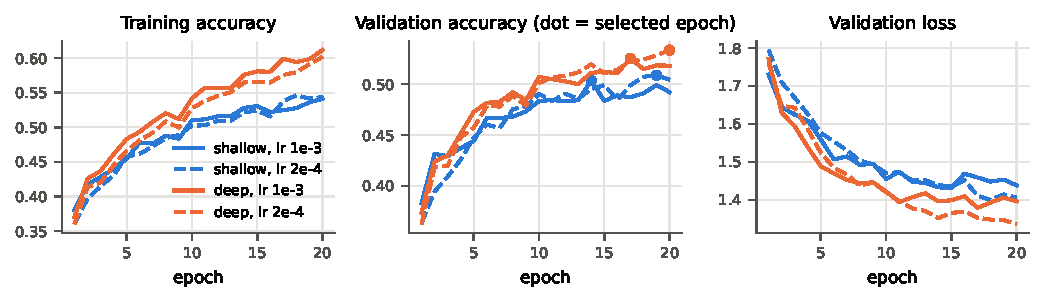
\includegraphics[width=\textwidth]{q1_curves}
\caption{Q1(a) training and validation curves for the four MLP runs. Blue is shallow and orange is deep; solid lines use lr $10^{-3}$, dashed lines lr $2{\times}10^{-4}$.}
\label{fig:q1}
\end{figure*}

\textbf{Result.} With the learning rate chosen on validation, the deep MLP reaches 52.59\% test accuracy and the shallow MLP 50.02\%.
Depth adds $+2.41$ points at lr $10^{-3}$ and $+2.57$ at $2{\times}10^{-4}$.
Changing the learning rate within one depth moves test accuracy by only $+0.67$ (shallow) and $+0.83$ (deep).
The depth effect is three times larger and has the same sign at both rates.
It is also about five times larger than our noise floor: the three Q2 MLP runs on permuted inputs are equivalent problems for an MLP and spread over 0.48 points.
The curves (\cref{fig:q1}) show that depth mainly raises the \emph{fit}.
The deep MLP's training-accuracy lead grows steadily, from 2 points at epoch 4 to 7 points at epoch 20, and its validation loss keeps falling, while the shallow MLP's validation loss stalls at 1.41--1.44.
So the shallow MLP is limited by representation, not step size.
Even so, depth explains little of the MLP's shortfall: the best MLP is still 19 points behind the CNN of Q2, which points to a missing spatial prior, tested directly in Q2.

\subsection{Learning structure before memorising}
\textbf{Setting.} The shallow MLP (1.55M parameters) is trained on a stratified 4,500-image subset, so it has about 345 parameters per example.
For 900 of these images (20\%) we replace the label with a uniformly drawn \emph{wrong} class.
We train for 100 epochs (3,600 updates) and log four quantities every epoch: accuracy on the 3,600 correctly labelled images, agreement with the \emph{wrong} label on the 900 relabelled images, agreement with their \emph{true} class, and clean validation accuracy.

\begin{figure}[t]
\centering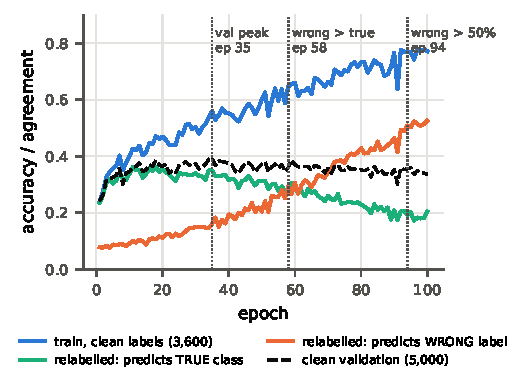
\includegraphics[width=\linewidth]{q1_memorization}
\caption{Q1(b) memorisation run. Before the validation peak the network predicts the true class of the relabelled images (green); afterwards it learns their wrong labels (orange).}
\label{fig:mem}
\end{figure}
\textbf{Evidence across training} (\cref{fig:mem}). In epochs 1--35, accuracy on correctly labelled images rises from 24\% to 56\% and validation from 24\% to its peak of 39.36\% (epoch 35).
Over the same epochs, the network predicts the \emph{true} class for up to 36.1\% of the relabelled images (epoch 18), although it was told something else for every one of them.
It agrees with the wrong label for only 8--16\% of them.
A network that only stored input--label pairs could not predict a class it was never shown for those images.
This behaviour therefore shows structure that transfers across images.
After the peak the pattern reverses.
Wrong-label agreement climbs to 52.56\%, overtakes true-class agreement at epoch 58 and passes 50\% at epoch 94.
True-class agreement falls to 20\%, and validation accuracy drops to 33.58\% while validation loss rises from 1.74 to 2.26.
\textbf{Conclusion.} Useful structure is learned \emph{before} memorisation: the validation peak comes 23 epochs before the wrong labels win and 59 epochs before most of them are memorised.
The two phases overlap, though, since wrong-label agreement already creeps from 8\% to 16\% before epoch 35.
Early stopping on clean validation (epoch 35) therefore captures most of the useful structure with little memorisation.

% ---------------------------------------------------------------- Q2
\section{Q2: Why the CNN wins}
\subsection{A fair CNN--MLP comparison}
\textbf{Fairness criterion, fixed before training.} The two models have the same parameter budget (within 1\%) and the same training conditions: data, scaling, optimiser and lr ($10^{-3}$), batch, 7,040 updates, seed, and validation-accuracy checkpointing.
Compute per update is \emph{not} matched (the CNN uses more), and we report this rather than hide it.
For that reason the MLP is the Q1 shallow model at lr $10^{-3}$, not the one at $2{\times}10^{-4}$.
\textbf{CNN} (1,563,180 parameters): three blocks of $3{\times}3$ convolution, ReLU and $2{\times}2$ max-pooling (16, 24, 48 channels), then dense layers $768{\to}1570{\to}216{\to}10$.
Most parameters sit in the dense layers so the budget matches the MLP's (1,553,842).
\textbf{Result} (\cref{tab:q2}). The CNN reaches 71.57\% test accuracy against the MLP's 49.35\%.
\textbf{Proposed reason:} the CNN reuses the same small filters across the image, which lets it build features from \emph{local neighbourhoods} of pixels (edges, textures, parts).
The MLP must learn every pixel position separately.

\begin{table}[t]
\centering\footnotesize
\setlength{\tabcolsep}{3pt}
\begin{tabular}{@{}llrcccc@{}}
\toprule
model & input & params & ep & test acc & conf.\ wrong & ECE\\
\midrule
MLP & clean & 1,553,842 & 14 & 49.35 & 0.424 & 0.014\\
MLP & pixel shuffle & 1,553,842 & 20 & 49.54 & 0.440 & 0.029\\
MLP & block shuffle & 1,553,842 & 15 & 49.06 & 0.425 & 0.017\\
CNN & clean & 1,563,180 & 12 & \textbf{71.57} & 0.660 & 0.100\\
CNN & pixel shuffle & 1,563,180 & 18 & 48.52 & 0.513 & 0.107\\
CNN & block shuffle & 1,563,180 & 12 & 62.10 & 0.589 & 0.097\\
\bottomrule
\end{tabular}
\caption{Q2 test results. Each model is trained \emph{and} tested with the same fixed transformation. ``conf.\ wrong'' is the mean max-softmax probability on errors; ECE uses 10 bins.}
\label{tab:q2}
\end{table}
\begin{figure}[t]
\centering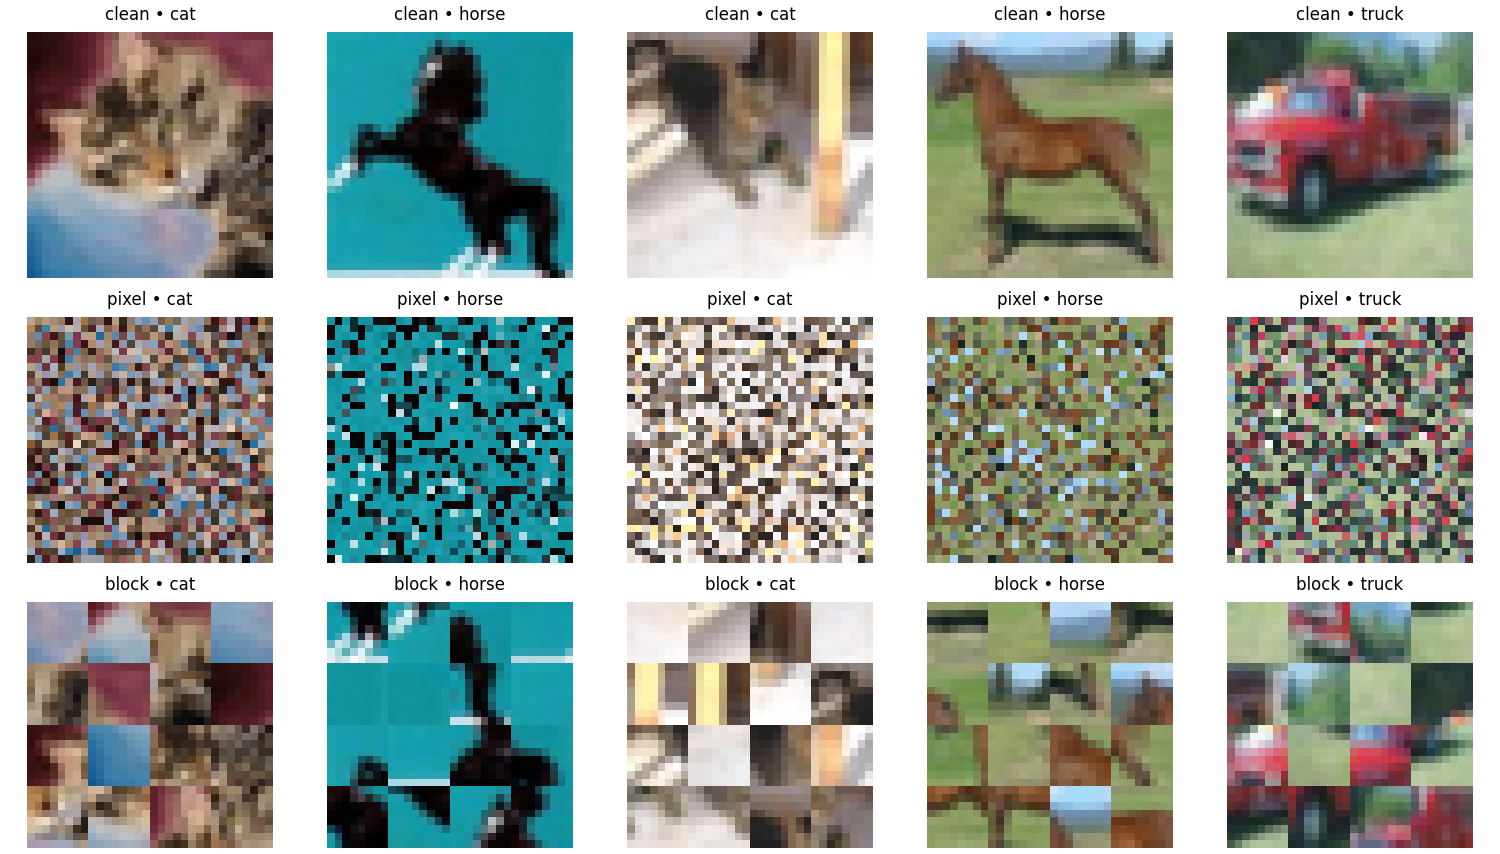
\includegraphics[width=\linewidth]{q2_inputs.png}
\caption{Q2 inputs (validation images): clean (top), after the fixed pixel permutation (middle) and after the fixed $8{\times}8$ block permutation (bottom).}
\label{fig:q2img}
\end{figure}
\begin{figure*}[t]
\centering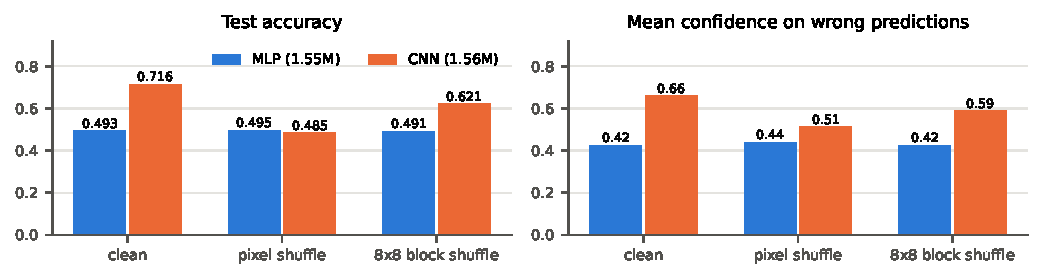
\includegraphics[width=0.92\textwidth]{q2_bars}
\caption{Q2 test accuracy (left) and mean confidence on wrong predictions (right) for the parameter-matched MLP and CNN, each trained and tested under the same input condition.}
\label{fig:q2}
\end{figure*}

\subsection{Destroying spatial structure}
\textbf{Modification.} One fixed random permutation of the 1,024 pixel positions is shared by the three colour channels and applied to the training, validation and test images.
Every pixel value is still present, but which pixels are neighbours is destroyed (\cref{fig:q2img}).
Both models are retrained from scratch.
\textbf{Expectation (stated before training).} The MLP should be \emph{unchanged} up to noise.
A fixed permutation only reorders its first-layer weights, so the learning problem is identical.
If the CNN's advantage comes from local neighbourhoods, the CNN should fall to the MLP's level.
\textbf{Observed.} The MLP gets 49.54\% (+0.19), as predicted.
The CNN falls by 23.05 points to 48.52\%, which is \emph{below} the MLP by 1.02 points (\cref{fig:q2}).
The entire 22.2-point advantage vanishes once neighbourhoods are scrambled, even though the CNN keeps the same filters, weight sharing and pooling.
This confirms the explanation from Q2(a): the advantage is in exploiting local spatial structure, not in having more parameters or capacity.
On permuted inputs the convolutions mix unrelated pixels, and the CNN overfits faster than the MLP (training accuracy 66\% against 55\% at the selected epoch).

\subsection{Local parts or global layout?}
\textbf{Two explanations.} The CNN could rely on (E1) local content, meaning textures and parts within small patches, or on (E2) the global arrangement of those parts.
\textbf{Experiment.} The image is cut into 16 blocks of $8{\times}8$ pixels, and one fixed permutation of the blocks is applied to all training, validation and test images.
Content inside each block survives, but the layout is scrambled (\cref{fig:q2img}, bottom row).
Under E1 the CNN should stay close to clean accuracy; under E2 it should fall to the pixel-shuffled level.
\textbf{Errors.} The CNN reaches 62.10\%, keeping 13.04 of its 22.22-point lead over the MLP (59\%), while the MLP is unchanged (49.06\%).
Local content therefore explains most of the advantage, but not all of it.
The remaining 9.5 points need intact layout, or are lost to artificial edges at block seams: the last convolution's receptive field is 18 pixels, wider than an $8{\times}8$ block.
By class, recall drops most for deer ($-18$ points), cat ($-11$) and truck ($-12$), and least for ship ($-1$) and automobile ($-7$).
This fits ship being recognisable from water and sky texture inside any block.
The most frequent error is cat$\leftrightarrow$dog in all six conditions, so scrambling adds errors but does not change the hardest pair.
\textbf{Confidence.} The CNN is overconfident in every condition.
Mean confidence minus accuracy is 0.100 (clean), 0.097 (block) and 0.107 (pixel), and it is still 51--66\% sure of its errors.
The MLP stays calibrated (ECE 0.014--0.029).
Overconfidence is therefore a property of how the CNN was trained (91\% training accuracy at the selected epoch), not of the input structure.
Confidence on errors does fall from 0.66 to 0.59 to 0.51 as structure is removed.
\textbf{Linking the three experiments.} The clean comparison establishes a 22-point gap at equal parameters.
Pixel shuffling shows the gap depends entirely on spatial neighbourhoods.
Block shuffling shows that about three fifths of it comes from content within $8{\times}8$ neighbourhoods, and the rest from their arrangement or seam artefacts.

% ---------------------------------------------------------------- Q3
\section{Q3: Autoencoders, denoising and class information}
\subsection{Bottleneck capacity}
The three autoencoders share an encoder ($3{\to}32{\to}64$ channels, $4{\times}4$ stride-2 convolutions, then a dense layer to the bottleneck) and a mirrored decoder with a sigmoid output.
They are trained for 20 epochs with MSE loss.
Only the bottleneck width changes: 16, 64 and 256 (a factor of 4 between sizes; 192$\times$, 48$\times$ and 12$\times$ smaller than the 3,072-value image).
Parameter counts differ only through the two dense layers next to the bottleneck (\cref{tab:q3}).
\textbf{Selection.} Validation MSE selects \textbf{bottleneck 256} (0.00267, 2.9$\times$ lower than 64), at its last epoch.
It has the lowest validation MSE at every epoch, and all three are still improving at epoch 20, so with MSE as the only criterion, more capacity always wins here.
Its test MSE is \textbf{0.00268}, matching validation, so there is no overfitting.

\begin{table}[t]
\centering\footnotesize
\setlength{\tabcolsep}{4pt}
\begin{tabular}{@{}rrcccc@{}}
\toprule
bottleneck & params & val MSE & test MSE & probe acc (\%)\\
\midrule
16 & 203,923 & 0.01650 & 0.01658 & 33.40\\
64 & 597,187 & 0.00779 & 0.00780 & 38.37\\
\textbf{256} & 2,170,243 & \textbf{0.00267} & \textbf{0.00268} & \textbf{41.82}\\
\bottomrule
\end{tabular}
\caption{Q3(a,c) autoencoders. The probe is a logistic regression ($C{=}1$) on standardised frozen codes, trained on the 45k training codes and tested on the test set.}
\label{tab:q3}
\end{table}

\subsection{Denoising}
\textbf{Corruption.} We add Gaussian noise ($\sigma{=}0.25$) and clip to $[0,1]$.
Reconstruction can plausibly undo this, because the noise is independent per pixel while images are spatially smooth.
\textbf{Protocol.} The denoiser has the same architecture as the selected 256 autoencoder.
It is trained on noisy training images as inputs with the clean images as targets, using \emph{no labels}.
The noise is drawn once per split with fixed seeds (26504, 26505, 26506 for train, validation and test).
It uses the same 20 epochs, and its checkpoint is chosen on clean-target validation MSE (epoch 19).
\textbf{Evaluation.} The fixed clean CNN from Q2(a) classifies the noisy test images and their reconstructions from the clean autoencoder (Q3(a), never trained on noise) and from the denoiser (\cref{fig:q3img,fig:q3}).

\begin{figure}[t]
\centering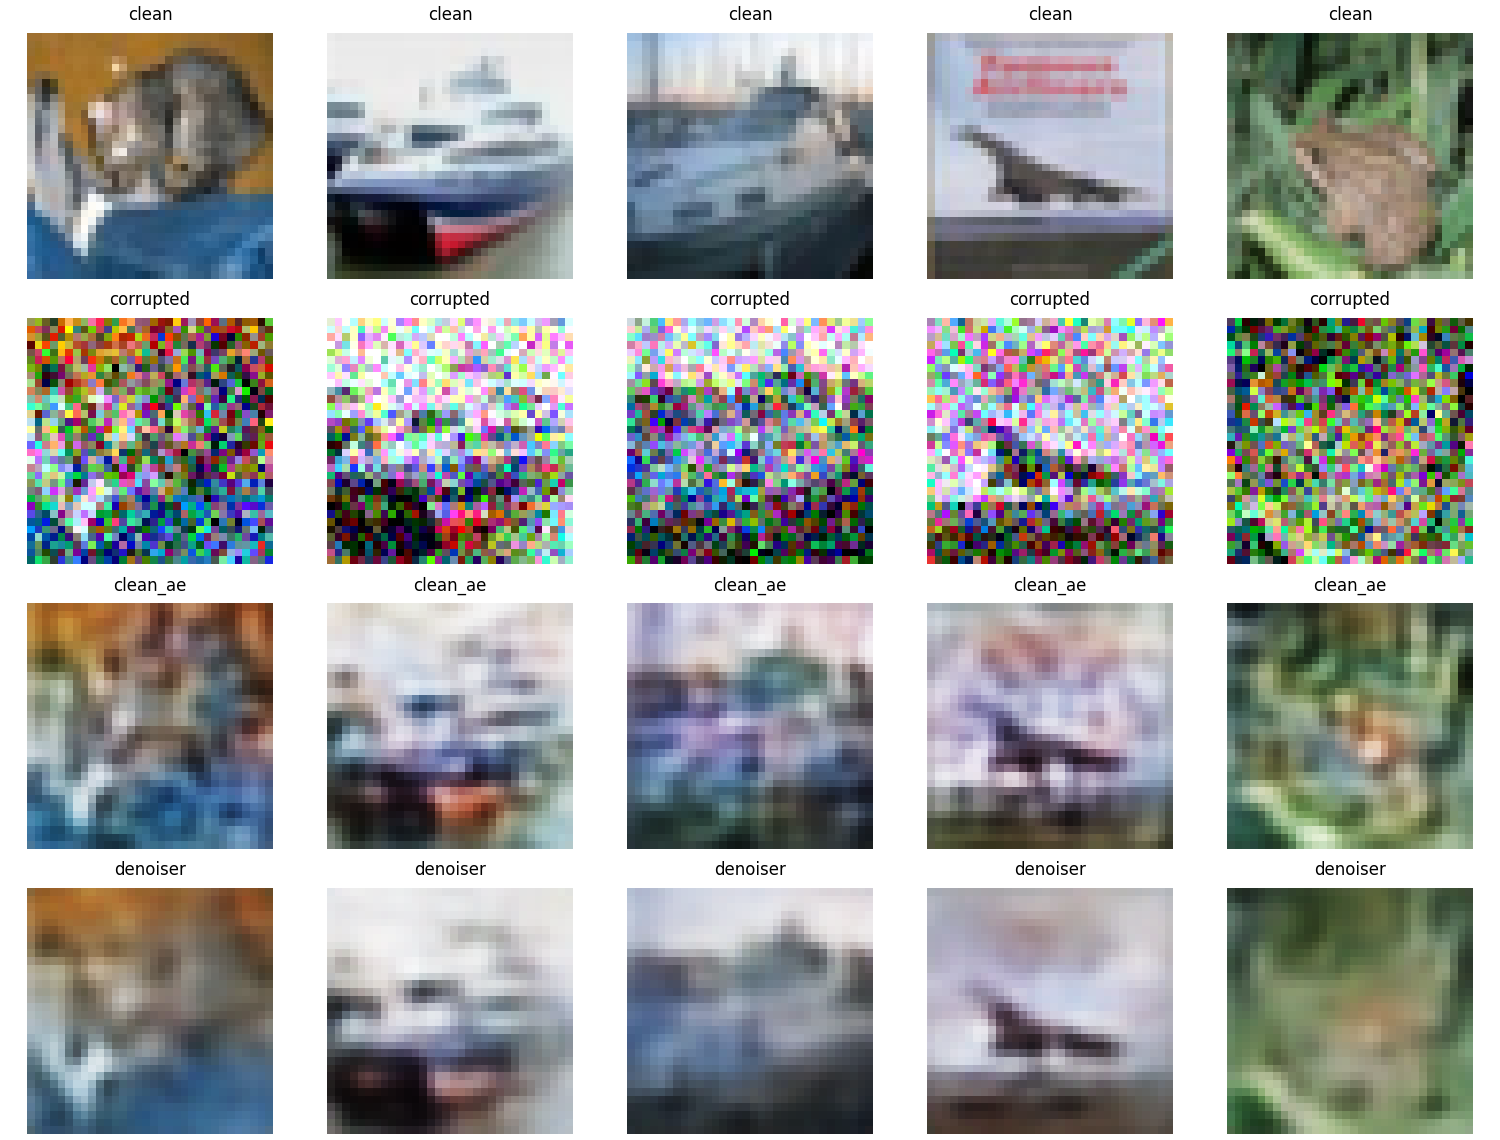
\includegraphics[width=\linewidth]{q3_reconstructions.png}
\caption{Q3(b) five test images, top to bottom: clean target, noisy input ($\sigma{=}0.25$), clean-autoencoder reconstruction, denoiser reconstruction.}
\label{fig:q3img}
\end{figure}
\begin{figure*}[t]
\centering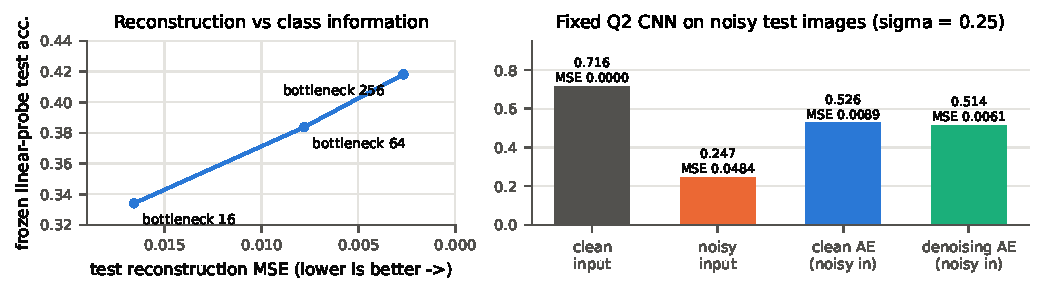
\includegraphics[width=0.92\textwidth]{q3_tradeoff}
\caption{Q3. Left: test reconstruction error against frozen linear-probe accuracy for the three bottlenecks. Right: the fixed Q2 CNN on clean, noisy and reconstructed test images (accuracy and MSE to the clean image).}
\label{fig:q3}
\end{figure*}

\textbf{Results.} Noise drops the CNN from 71.57\% to 24.70\% while its mean confidence stays at 82\%, a severely overconfident failure (ECE 0.58).
The denoiser cuts pixel error to 0.0061, 31\% below the clean autoencoder's 0.0089.
Yet it gives \emph{slightly lower} CNN accuracy: 51.38\% against 52.65\%.
Both reconstructions bring ECE down to about 0.2.
\textbf{Decision.} Denoising recovers part of the information the classifier needs, but not all of it: 57\% of the 46.9 points lost to noise (59\% for the clean autoencoder), leaving it 20 points below clean images.
The recovery comes from the \emph{bottleneck}, not from learning to denoise.
An autoencoder that never saw noise does as well, because squeezing the image through 256 values removes most of the independent per-pixel noise.
The reconstructions in \cref{fig:q3img} show why lower MSE does not mean better classification.
The denoiser buys its lower error by smoothing more strongly, and in doing so erases edges and texture the CNN depends on (e.g.\ the frog, rightmost, almost disappears).
Pixel MSE rewards average colour; the CNN needs high-frequency detail.
One limitation: we did not measure the CNN on reconstructions of \emph{clean} images, so the accuracy lost to the autoencoder itself is not isolated.

\subsection{Class information versus reconstruction}
Without fine-tuning, we freeze each encoder and fit a linear probe on its standardised codes (\cref{tab:q3}).
\textbf{Within the bottleneck family the two measures agree.} Lower MSE goes with higher probe accuracy at every step: 33.4\%, 38.4\% and 41.8\% (\cref{fig:q3}, left).
\textbf{But they agree weakly and not beyond this family.} A $6.2{\times}$ reduction in MSE buys only 8.4 points of probe accuracy.
The best code (41.8\%) is linearly \emph{less} informative than the raw-pixel MLP of Q1 (49.4\%, a nonlinear model).
It is far below the CNN features that a linear SVM reads at 71.7\% (Q4).
Q3(b) also gives a direct counter-example: the denoiser has lower MSE but its output carries less class information for the CNN.
\textbf{Conclusion.} Reconstruction quality and class information are only loosely linked.
The reconstruction objective spends capacity on reproducing colour and background accurately, which matters for MSE but carries little class signal.

% ---------------------------------------------------------------- Q4
\section{Q4 (bonus): SVMs and clustering on CNN features}
\subsection{Kernel and $C$}
\textbf{Fixed representation.} We use the 216-dimensional penultimate ReLU activations of the clean Q2 CNN, standardised with training statistics.
It stays unchanged for all of Q4.
\textbf{Subset.} Because of cost, every SVM is fitted on one stratified 3,000-image training subset (300 per class, seeded, saved in \texttt{split.npz}), fixed before any model selection.
Validation always uses the full 5,000-image validation set.
We sweep linear, RBF (\texttt{gamma=scale}) and degree-2 polynomial kernels over $C\in\{0.01,0.1,1,10,100\}$, five orders of magnitude (\cref{tab:q4,fig:q4}).

\begin{table}[t]
\centering\footnotesize
\setlength{\tabcolsep}{3.4pt}
\begin{tabular}{@{}lrccc@{\hskip 8pt}lrccc@{}}
\toprule
kernel & $C$ & train & val & SV & kernel & $C$ & train & val & SV\\
\midrule
linear & 0.01 & 93.20 & \textbf{73.44} & .447 & rbf & 10 & 97.23 & 72.80 & .381\\
linear & 0.1 & 95.50 & 73.00 & .302 & rbf & 100 & 99.80 & 71.30 & .384\\
linear & 1 & 98.13 & 71.82 & .264 & poly & 0.01 & 30.93 & 27.82 & .982\\
linear & 10 & 99.43 & 70.60 & .265 & poly & 0.1 & 71.93 & 59.86 & .806\\
linear & 100 & 99.77 & 70.40 & .263 & poly & 1 & 89.67 & 70.50 & .557\\
rbf & 0.01 & 86.30 & 71.30 & 1.000 & poly & 10 & 95.47 & 71.46 & .405\\
rbf & 0.1 & 90.50 & 72.58 & .747 & poly & 100 & 99.07 & 69.58 & .386\\
rbf & 1 & 93.97 & 73.16 & .485 & & & & &\\
\bottomrule
\end{tabular}
\caption{Q4(a) full sweep: training accuracy (3,000-image subset), validation accuracy (5,000) in \%, and the fraction of training points that are support vectors.}
\label{tab:q4}
\end{table}
\begin{figure*}[t]
\centering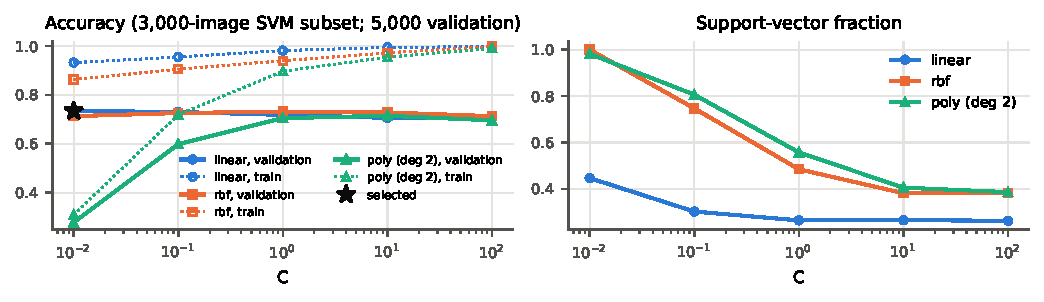
\includegraphics[width=\textwidth]{q4_sweep}
\caption{Q4(a) validation accuracy (solid), training accuracy (dotted) and support-vector fraction against $C$ for each kernel. The star marks the selected model.}
\label{fig:q4}
\end{figure*}

\textbf{Selected: linear kernel, $C{=}0.01$} (validation 73.44\%).
\textbf{Test accuracy: 71.73\%}, the single evaluation on the official test set.
\textbf{Behaviour across the sweep.}
\emph{Linear, overfitting as $C$ grows:} training accuracy rises from 93.2\% to 99.8\% while validation falls from 73.4\% to 70.4\%.
The support-vector fraction drops from 0.45 to 0.26 as the margin narrows around the training points.
\emph{RBF:} at $C{=}0.01$ every training point is a support vector (fraction 1.00).
That is the widest-margin, most regularised model, already at 71.3\%; RBF peaks at $C{=}1$ (73.16\%) and overfits by $C{=}100$ (99.8\% train, 71.3\% validation).
\emph{Polynomial, clear underfitting at small $C$:} 30.9\% training and 27.8\% validation at $C{=}0.01$, with 98\% support vectors.
It needs $C\ge1$ to become competitive.
All three kernels peak within 0.3--2 points of each other (73.4, 73.2, 71.5), so these features are already close to linearly separable and $C$ matters more than the kernel.
The linear winner beats RBF by only 0.28 points, which is 14 validation images.
\textbf{Caveats.} Training accuracy is inflated, because the CNN that produces the features was trained on these same images.
Validation is slightly optimistic, because it also selected the CNN checkpoint.
The test result is clean: 71.73\% essentially equals the CNN's own softmax head (71.57\%), so the representation, not the classifier on top, is what limits accuracy.

\subsection{Difficult pairs and the boundary}
The three pairs with the most mutual test errors are cat/dog (342), automobile/truck (193) and bird/deer (180).
For each pair we take the one-vs-one decision function and show the three training support vectors and the three test images of that pair closest to its zero level (\cref{fig:svm}).
The signed scores are tiny: $|f|\le0.02$ for the support vectors and $\le0.008$ for the test images.
With $C{=}0.01$ the margin is wide and 45\% of training points are support vectors, so these classes overlap \emph{inside} the margin rather than meeting at a clean edge.

\begin{figure*}[t]
\centering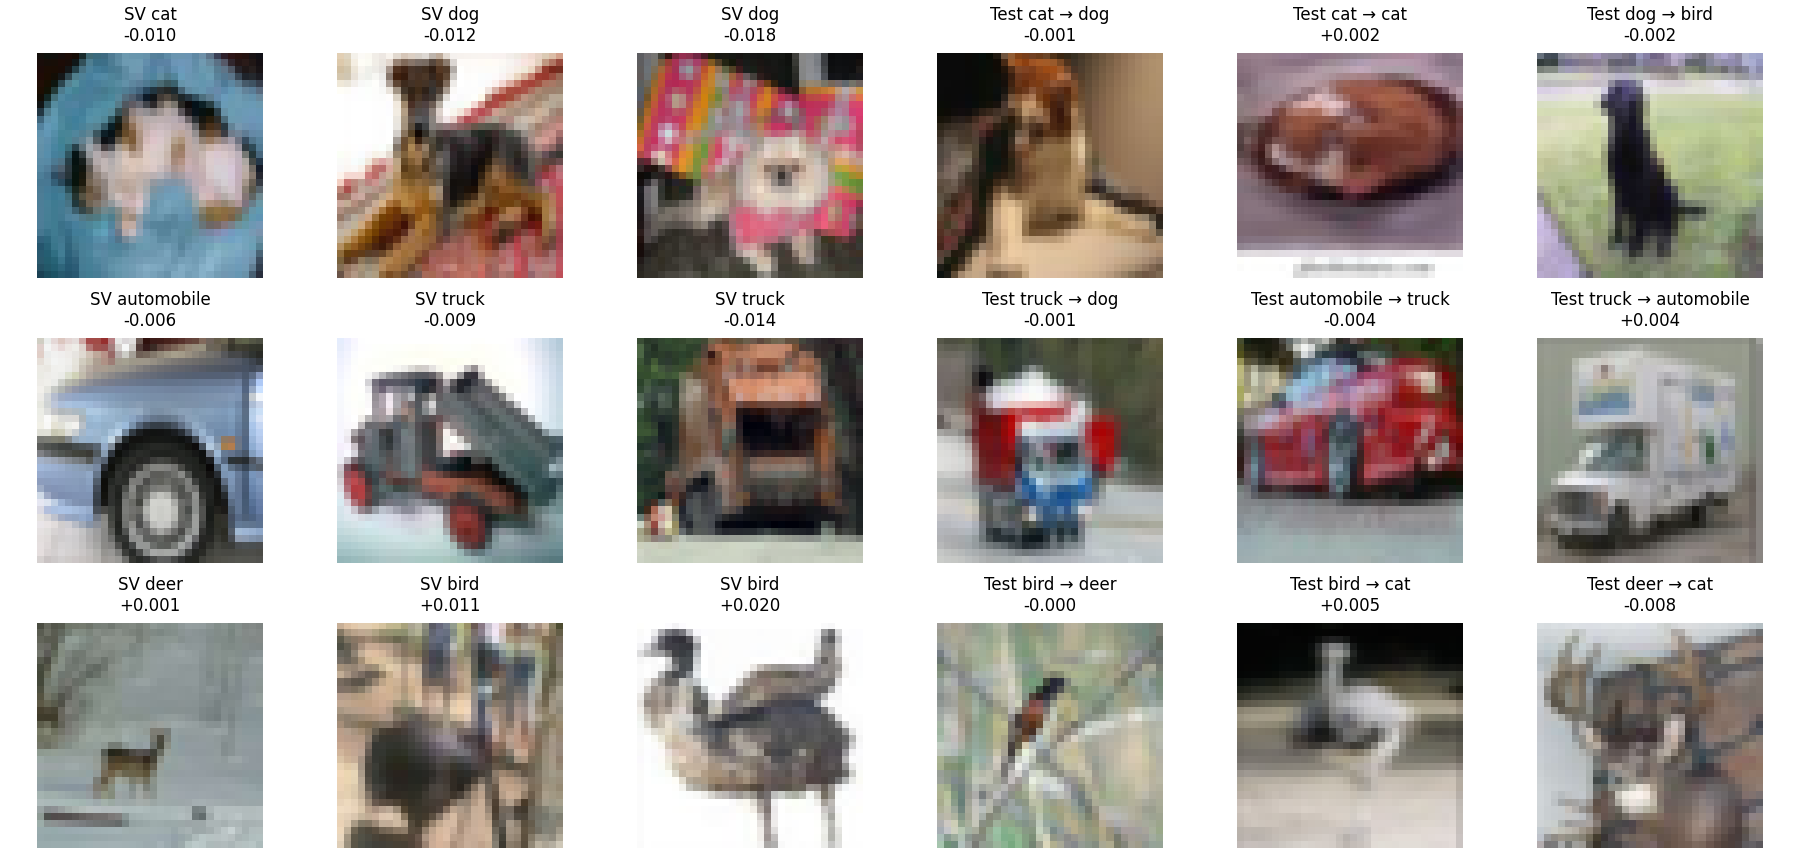
\includegraphics[width=0.86\textwidth]{q4_boundaries.png}
\caption{Q4(b) one row per difficult pair (cat/dog, automobile/truck, bird/deer). Left three: training support vectors nearest the pairwise boundary, with their decision score. Right three: test images nearest the boundary, with true class $\to$ final multiclass prediction and pairwise score.}
\label{fig:svm}
\end{figure*}

\textit{Cat/dog.} The support vectors include a cat on a blue blanket and a fluffy small dog on a patterned rug.
In both, pose and fur colour, not face shape, dominate the image.
A cat in an upright pose with a tan face sits at $-0.001$ and is predicted dog.
A curled cat on a bed sits at $+0.002$, on the correct side.
\textit{Automobile/truck.} The support vectors are a close-up of a car's wheel arch, a toy dump truck and a refuse truck seen head-on.
At $32{\times}32$, shared parts (wheels, grilles) dominate.
A red car ($-0.004$) and a white box truck ($+0.004$) land on opposite wrong sides.
\textit{Bird/deer.} The support vectors are a small deer in a large snowy scene, a dark bird against clutter and a large flightless bird.
They are atypical members of each class, and in the deer image the background dominates.
A small bird among branches scores $-0.000$ and becomes deer.
\textbf{Link to the test errors.} Four of the nine boundary test images end up predicted as a \emph{third} class: dog$\to$bird, truck$\to$dog, bird$\to$cat and deer$\to$cat.
Points near one pairwise boundary are thus often in a region where several classes meet.
This is why the confusions concentrate among the animal classes, and why a $k$-means ``animal'' cluster appears below.

\subsection{Clustering versus classification}
\textbf{Method.} $k$-means~\cite{lloyd1982kmeans} with 5 initialisations is fitted on the 45k training features, with no labels.
$k\in\{8,10,15,20\}$ is chosen by silhouette on the \emph{unlabelled} validation features: 0.135, 0.123, 0.102, 0.096.
\textbf{$k{=}8$} wins; it is the smallest value tried, so the silhouette optimum may lie lower still.
The fitted model assigns test features to clusters, and test labels are used only afterwards.
\textbf{Test result: ARI 0.346, NMI 0.493}, purity 59\% (\cref{tab:cont}).

\begin{table}[t]
\centering\footnotesize
\setlength{\tabcolsep}{3.2pt}
\begin{tabular}{@{}lrrrrrrrr@{}}
\toprule
class $\backslash$ cluster & 0 & 1 & 2 & 3 & 4 & 5 & 6 & 7\\
\midrule
airplane & 41 & 133 & 1 & 17 & \textbf{687} & 2 & 11 & 108\\
automobile & 100 & 72 & 8 & 11 & 9 & 0 & \textbf{757} & 43\\
bird & 6 & \textbf{620} & 61 & 133 & 157 & 10 & 3 & 10\\
cat & 11 & 316 & 71 & \textbf{572} & 13 & 5 & 4 & 8\\
deer & 0 & \textbf{838} & 53 & 40 & 13 & 49 & 1 & 6\\
dog & 7 & 209 & 8 & \textbf{740} & 8 & 20 & 1 & 7\\
frog & 2 & 159 & \textbf{764} & 58 & 6 & 1 & 3 & 7\\
horse & 15 & 320 & 3 & 102 & 4 & \textbf{550} & 2 & 4\\
ship & 11 & 87 & 2 & 13 & 43 & 1 & 24 & \textbf{819}\\
truck & \textbf{753} & 78 & 10 & 13 & 20 & 1 & 86 & 39\\
\midrule
cluster size & 946 & 2832 & 981 & 1699 & 960 & 639 & 892 & 1051\\
\bottomrule
\end{tabular}
\caption{Q4(c) test contingency table (rows: true class, 1,000 each). Bold marks each class's largest cluster.}
\label{tab:cont}
\end{table}
\begin{figure}[t]
\centering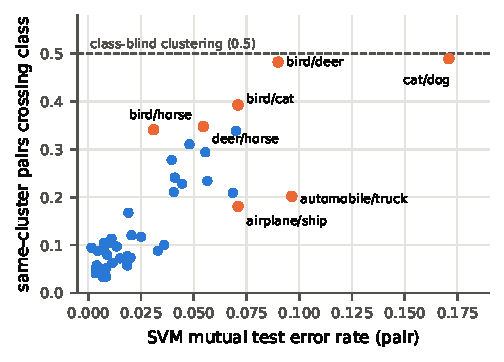
\includegraphics[width=\linewidth]{q4_pairs}
\caption{Q4(c) all 45 class pairs. $x$: SVM mutual test error rate. $y$: among test pairs from the two classes that share a cluster, the fraction with different classes. A clustering blind to class gives 0.5.}
\label{fig:pairs}
\end{figure}

\textbf{Measure.} For each class pair we compare the SVM's mutual error rate $(n_{ab}{+}n_{ba})/2000$ with clustering's \emph{cross-class fraction}: among test pairs from the two classes that land in the same cluster, the share drawn from different classes (\cref{fig:pairs}).
Over all 45 pairs the two methods largely agree (Spearman $\rho{=}0.82$).
Cat/dog is the hardest pair for both (17.1\% error; cross-class fraction 0.49).
\textbf{Disagreement 1, bird/deer.} The SVM separates them well (9.0\% mutual error), but clustering treats them as one group.
The cross-class fraction is 0.483, almost exactly the 0.5 of a clustering that ignores class, because 838 deer and 620 birds share cluster 1.
That cluster is a 2,832-image ``animal'' group that also holds 320 horses and 316 cats.
Deer/horse (5.5\% against 0.35) and bird/horse (3.1\% against 0.34) show the same pattern.
\textbf{Disagreement 2, automobile/truck}, in the opposite direction.
It is the SVM's second-hardest pair (9.65\%, rank 2 of 45), yet clustering separates the two well: cross-class fraction 0.20 (rank 15), with 757 automobiles in cluster 6 and 753 trucks in cluster 0.
\textbf{Interpretation.} $k$-means follows the directions of largest Euclidean spread.
In this representation those separate vehicles by type but merge animals photographed in natural scenes.
The supervised SVM can instead use low-variance directions that still predict the class (bird against deer), while its errors on automobile/truck come from the few boundary images (\cref{fig:svm}) rather than from a merged mass.
So \emph{classification says bird and deer are distinct; clustering says they are not}.
For automobile and truck, classification struggles at the boundary while their bulk forms separate clusters.

% ---------------------------------------------------------------- end
\section{Conclusion and limitations}
At an equal parameter budget, the CNN's 22-point advantage over the MLP depends entirely on neighbouring pixels being neighbours, mostly within $8{\times}8$ patches.
MLP depth helps far less.
Given noisy labels, an MLP learns transferable structure before it memorises.
Autoencoder reconstruction quality is a weak and sometimes misleading proxy for class information.
Frozen CNN features are close to linearly separable, yet their unsupervised geometry groups classes differently from the labels.
\textbf{Limitations.} Every number comes from one seed and one split; the 0.48-point spread of the equivalent MLP runs gives a rough noise scale.
The SVMs use a 3,000-image subset.
\textbf{Reproduction.}
\texttt{python -u run.py --device cuda --roll M26ECM503 --data data --out results}
trains everything and writes \texttt{metrics.json}, \texttt{split.npz} and the image montages.
\texttt{python make\_report\_figures.py --results results --out report/figs} redraws the plots.
The repository README lists the exact environment (Python 3.12, PyTorch 2.7.1, scikit-learn 1.6.1).

{\small
\bibliographystyle{ieeenat_fullname}
\bibliography{main}
}
\end{document}
